\documentclass[11pt,a4paper]{report}

\usepackage[utf8]{inputenc}
\usepackage{amsmath}
\usepackage{graphicx}
\usepackage{gensymb}
\usepackage{tikz}
\usetikzlibrary{positioning}
\usepackage{geometry}
\geometry{
    left=2cm,
    right=0.64cm,
    top=0.64cm,
    bottom=2cm
}
\usepackage{multicol}
\setlength{\columnsep}{1cm}
\graphicspath{ {images/} }

\begin{document}

\chapter{Semester 2 Examination 2014-2015\\CZ4034 Information Retrieval}

\begin{multicols*}{2}

\section{Question 1}

\noindent \textbf{Question 1a}

\noindent \textbf{(i)} Posting list: It is a list of document IDs that contain a specific dictionary term, and is used in inverted index. The posting list needs to be a variable size list so that new documents can be added easily to the list.

\begin{center}
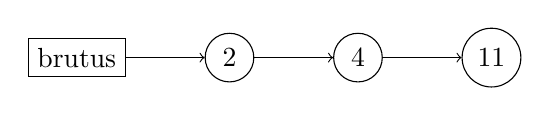
\begin{tikzpicture}[
squarenode/.style={rectangle, draw=black, thin},
roundnode/.style={circle, draw=black, thin},
]
%Nodes
\node[squarenode](brutus){brutus};
\node[roundnode](2)[right=of brutus]{2};
\node[roundnode](4)[right=of 2]{4};
\node[roundnode](11)[right=of 4]{11};

\draw[->](brutus.east) -- (2.west);
\draw[->](2.east) -- (4.west);
\draw[->](4.east) -- (11.west);
\end{tikzpicture}
\end{center}

\noindent \textbf{(ii)} Biword index: We use two consecutive words as dictionary pharases, instead of using unigram which treat each words as dictionary terms. For example, if we have the following sentence:
\begin{center}
\verb|I am a boy|
\end{center}
\noindent Then our dictionary phrases are: \verb|I am|, \verb|am a|, \verb|a boy|. \\

\noindent \textbf{(iii)} Stemming: Reduce terms to their “roots”, by crude chopping. For example:
\begin{itemize}
    \item automates automatic automation $\rightarrow$ automat
    \item democrats $\rightarrow$ democrat
    \item democratized $\rightarrow$ democrat
\end{itemize}

\noindent \textbf{Question 1b}

\noindent \verb|one$|, \verb|ne$o|, \verb|e$on|, \verb|$one|, \verb|two$|, \verb|wo$t|, \verb|o$tw|, \verb|$two|, \verb|three$|, \verb|hree$t|, \verb|ree$th|, \verb|ee$thr|, \verb|e$thre|, \verb|$three|\\

\noindent \textbf{Question 1c}

\begin{center}
\begin{tabular}{ | l | l  l  l  l  l |}
    \hline
      &   & w & o & r & k \\
    \hline
      & 0 & 1 & 2 & 3 & 4 \\
    w & 1 & 0 & 1 & 2 & 3 \\
    a & 2 & 1 & 1 & 2 & 3 \\
    l & 3 & 2 & 2 & 2 & 3 \\
    k & 4 & 3 & 3 & 3 & \textbf{2} \\
    \hline
\end{tabular}
\end{center}

\noindent \textbf{Question 1d}

\begin{itemize}
    \item DocA: love lord great
    \item DocB: great love lord gene
    \item DocC: love lord gentle
\end{itemize}

\noindent First we sort all vocabulary

\begin{center}
\verb|gene, gentle, great, lord, love|
\end{center}

\noindent Then, we add length of string the the front of each word. the pointer points to every 2 words, since block(k=2).

\begin{center}

\verb| 4gene6gentle5great4lord4love|
\verb|a           b          c    |
\end{center}

\noindent The data structure of the index is:

\begin{center}
\begin{tabular}{ | l | l | l |}
    \hline
    Frequency & Postings pointer & Term pointer \\
    \hline
    1 & $p_1$ & a\\
    1 & $p_2$ & \\
    2 & $p_3$ & b\\
    3 & $p_4$ & \\
    3 & $p_5$ & c\\
    \hline
\end{tabular}
\end{center}

\noindent Posting list:
\begin{center}
\begin{tabular}{ | l | l |}
    \hline
    Postings pointer & postings \\
    \hline
    $p_1$ & DocB\\
    $p_2$ & DocC\\
    $p_3$ & DocA, DocB\\
    $p_4$ & DocA, DocB, DocC\\
    $p_5$ & DocA, DocB, DocC\\
    \hline
\end{tabular}
\end{center}

\noindent Optimisation for posting list includes recording the gaps between document ID rather than the exact document ID.\\

\noindent Since front coding is only applied for words with long common prefix, it does not apply in this case.\\

\noindent \textbf{Question 1e}

\noindent Not in syllabus \\

\noindent \textbf{Question 1f}

\noindent The champion list contains a set of $n$ documents with the highest weights for the given term. The number $n$ can be chosen to be different for each term and is often higher for rarer terms. The weights can be calculated by for example TF-IDF. At query time, we only compute scores for documents in the champion list for some query terms.

\section{Question 2}

\begin{center}
Q: \verb|apple google|\\
Doc1: \verb|facebook google google google|\\
Doc2: \verb|google apple apple facebook|\\
\end{center}

\noindent \textbf{Question 2a}

\noindent \verb|apple|. The document frequency for \verb|google| is 2, which makes the $\text{idf}_{\text{google}}=0$. Without any calculation, we can say that the term \verb|google| is a common term and hence can be removed from the query. On the other hand, the term \verb|apple| does not appear in every documents, so the term contains more information.\\

\noindent \textbf{Question 2b}

\noindent\underline{Term frequency and idf}:

\begin{center}
\begin{tabular}{|l | l | l | l | l|}
    \hline
    term     & tf of Doc1 & tf of Doc2 & df & idf \\
    \hline
    apple    & 0 & 2 & 1 & 0.3010\\
    facebook & 1 & 1 & 2 & 0\\
    google   & 3 & 1 & 2 & 0\\
    \hline
\end{tabular}
\end{center}
$$ idf = log(N / df) $$
$$ N = \text{no. of docs} = 2$$

\noindent \underline{For document, \textit{lnc}.}\\

\noindent Doc1

\begin{center}
\begin{tabular}{| l | l | l | l | l | l | l|}
    \hline
    term     & tf & l & n & ln & c & lnc\\
    \hline
    apple    & 0 & 0 & 1 & 0 & 0 & 0\\
    facebook & 1 & 1 & 1 & 1 & 0.5606 & 0.5606\\
    google   & 3 & 1.477 & 1 & 1.477 & 0.5606 & 0.8280\\
    \hline
\end{tabular}
\end{center}

\begin{equation*}
\begin{split}
l                   &= 1 + log(tf)\\
l_{\text{facebook}} &= 1 + log(1) = 1\\
l_{\text{google}}   &= 1 + log(3) = 1.477
\end{split}
\end{equation*}

\begin{equation*}
\begin{split}
n &= 1 \\
l_{\text{facebook}} n &= 1 \\
l_{\text{google}}n &= 1.477
\end{split}
\end{equation*}

$$c = \frac{1}{\sqrt{1^2 + 1.477^2}} = 0.5606$$

\noindent Similary, for Doc2

\begin{center}
\begin{tabular}{|l | l | l | l |}
    \hline
    term     & tf & l & c \\
    \hline
    apple    & 2 & 1.301 & 0.677 \\
    facebook & 1 & 1 & 0.520\\
    google   & 1 & 1 & 0.520\\
    \hline
\end{tabular}
\end{center}

\noindent \underline{For query, \textit{ltc}.}
\begin{center}
\begin{tabular}{|l | l | l | l | l | l |l |}
    \hline
    term     & tf & l & t & lt & c & ltc\\
    \hline
    apple    & 1 & 1 & 0.3010 & 0.3010 & 3.322 & 1\\
    facebook & 0 & 0 & 0 & 0 & 3.322 & 0\\
    google   & 1 & 1 & 0 & 0 & 3.322 & 0\\
    \hline
\end{tabular}
\end{center}

\begin{equation*}
\begin{split}
t_{\text{apple}} & = \log(N/df), \text{where }N = \text{no. of doc} = 2 \\
& = \log(2/1) \\
& = 0.3010 \\
c &= \frac{1}{\sqrt{0.3010^2 + 0^2 + 0^2}} \\
  &= 3.322
\end{split}
\end{equation*}

\noindent The cosine similarities:
\begin{equation*}
\begin{split}
format &= (apple, facebook, google)\\
Q &= (1, 0, 0)\\
doc1 &= (0, 0.5606 ,0.8280)\\
doc2 &= (0.677, 0.520, 0.520)\\
\text{cosine}(Q, doc1) &= 0\\
\text{cosine}(Q, doc2) &= 0.677\\
\end{split}
\end{equation*}

\noindent Doc2 is ranked higher than Doc1.\\

\noindent \textbf{Question 2c}

\noindent \underline{For document, \textit{ntc}.}

\noindent Doc1

\begin{center}
\begin{tabular}{|l | l | l | l|}
    \hline
    term     & tf & t & c \\
    \hline
    apple    & 0 & 0 & 0 \\
    facebook & 1 & 0 & 0 \\
    google   & 3 & 0 & 0 \\
    \hline
\end{tabular}
\end{center}

\noindent Doc2

\begin{center}
\begin{tabular}{|l | l | l | l|}
    \hline
    term     & tf & t & c \\
    \hline
    apple    & 2 & 0.602 & 1 \\
    facebook & 1 & 0 & 0\\
    google   & 1 & 0 & 0\\
    \hline
\end{tabular}
\end{center}

\noindent \underline{For query, \textit{atc}.}

\begin{center}
\begin{tabular}{|l | l | l | l | l |}
    \hline
    term     & tf & a & t & c \\
    \hline
    apple    & 1  & 1 & 0.301 & 1\\
    facebook & 0  & 0 & 0 & 0\\
    google   & 1  & 1 & 0 & 0 \\
    \hline
\end{tabular}
\end{center}

\noindent The cosine similarities:

$$\text{cosine}(Q, doc1) = 0$$
$$\text{cosine}(Q, doc2) = 1$$

\noindent Doc2 is ranked higher than Doc1\\

\noindent \textbf{Question 2d}

\noindent Netscore for both documents:
$$\text{netscore}(Doc1) = g(Doc1) + cosine(Doc1, Q) = 0.9$$
$$\text{netscore}(Doc2) = g(Doc2) + cosine(Doc2, Q) = 0.777$$
\noindent Now, Doc1 is ranked higher than Doc2 \\

\noindent \textbf{Question 2e}

\noindent Not in syllabus \\

\noindent \textbf{Question 2f}

\noindent We always consider a document as a piece of unstructured text. However, document usually have multiple parts, with special semantics. For example, a twitter post contains author, creation data, and language. These are the metadata of documents. By having these metadata, we can implement filter or range retrieval function. Hence, the retrieval results can be narrowed down using specific criteria to achieve better retrieval results.

\section{Question 3}

\noindent \textbf{Question 3a}

\noindent Since this is supervised learning with labelled training data, we should use kNN. k-means clustering is an unsupervised clustering algorithm. \\

\noindent \textbf{Question 3b}

\noindent Not in syllabus \\

\noindent \textbf{Question 3c}

\noindent Documents in the same cluster are similar, where the similarity is defined by the dot product of the Euclidean distance or cosine similarity in most cases. The document with the same concept but not using the same term are likely to have a lot of other common terms like transfer, money, interest, which will put them into the same cluster. \\

\noindent \textbf{Question 3d}

\noindent We rephrase the question as, what is the probabilty of SQ KrisFlyer members, given that the members are Premiermiles card hold- ers.

$$P(\text{card} | \text{SQ}) = 0.5$$
$$P(\text{SQ}) = 0.01$$
$$P(\text{card}) = 0.9$$

$$P(\text{SQ} | \text{card}) = \frac{P(\text{card} | \text{SQ}) P(\text{SQ})}{P(\text{card})} = 0.55\%$$

\noindent If we send the advertisement to all Premiermiles customers, only 0.55\% of them would probably be interested on the advertisment. So we better don't send the advertisment out. \\

\noindent \textbf{Question 3e}

\noindent \textbf{(i)} Since every type of card is represented as a list of features (the kinds of services they provide), we can measure the similarity between two cards. If two cards are similar, it means they offer similar services. Hence, the bank could probably combine similar credit cards to avoid confusion. \\

\noindent \textbf{(ii)}

\begin{equation*}
\begin{split}
    \text{Distance} &= \sqrt{(0.81 - 0.5)^2 + (0.93 - 0.79)^2 + (0.6)^2}\\
    &= 0.690
\end{split}
\end{equation*}

\noindent \textbf{Question 3f}

\noindent \textbf{(i)} Not in syllabus\\

\noindent \textbf{(ii)} Not in syllabus

\section{Question 4}

\noindent \textbf{Question 4a}

\noindent \textbf{(i)} TRUE.\\

\noindent \textbf{(ii)} TRUE.\\

\noindent \textbf{(iii)} TRUE.\\

\noindent \textbf{(iv)} TRUE.\\

\noindent \textbf{(v)} TRUE.\\

\noindent \textbf{(vi)} TRUE.\\

\noindent \textbf{(vii)} TRUE.\\

\noindent \textbf{(viii)} FALSE.\\

\noindent \textbf{(ix)} FALSE.\\

\noindent \textbf{(x)} UNKNOWN\\

\noindent \textbf{Question 4b}

\scriptsize
\begin{center}
\begin{tabular}{ |l|l|l|l| }
    \hline
            & PhD       & Not Phd     & Total \\
    \hline
    Inside  & $A = 350$ & $B = 20601$ & $A+B=20951$ \\
    Outside & $C = 350$ & $D = 12099$ & $C+D=12449$ \\
    Total   & $A+C=700$ & $B+D=32700$ & $N=33400$ \\
    \hline
\end{tabular}
\end{center}
\normalsize

\begin{equation*}
\begin{split}
   \chi^2(t,c) &= \frac{N\times (AD - BC)^2}{(A+B) \times (C+D) \times (A+C) \times (B+D)} \\
   &= \frac{33400\times ((350 \times 12099) - (20601 \times 350))^2}{700\times 32700 \times 20951 \times 12449}\\
   &= 49.54 > 10.83
\end{split}
\end{equation*}

\noindent \textbf{Question 4c}

\noindent \textbf{(i)}
$$P(\text{Male}) = \frac{120}{200} = 0.60$$

\noindent \textbf{(ii)}
$$P(\text{foreign} \cap \text{female}) = \frac{30}{200}\cdot \frac{80}{200}=0.06$$

\noindent \textbf{(iii)}
$$P(\text{europe} \cap \text{male}) = \frac{15}{200}\cdot \frac{120}{200}=0.045$$

\noindent \textbf{Question 4d}

\noindent \textbf{(i)} Hard clustering means every data is only belong to one cluster and soft clustering means every data can belong to more than one clusters\\

\noindent \textbf{(ii)} Hard clustering, we have algorithm such as k-mean clustering to solve the problem.\\

\noindent \textbf{(iii)} I will recommend the top-down approach. To use top-down approach, we would split a group of students into separate groups until we are satisfied. It is easier to use simple rules to split them into groups(e.g. split by gender, age, hairstyle, ..). The bottom up approach is more tedious as the mentor will have to compare 1 student to every other student at the start.

\end{multicols*}
\end{document}
